\documentclass[
    11pt,
    a4paper,
    egregdoesnotlikesansseriftitles,
    toc=chapterentrywithdots,
    twoside,openright,
    titlepage,
    parskip=half,
    headings=normal,  % reduces heading size
    listof=totoc,
    bibliography=totoc,
    index=totoc,
    captions=tableheading,  % caption below table
    chapterprefix,
    listof=flat,
    final
]{scrbook}


% details about your thesis
\newcommand{\titel}{Enablement of Kubernetes Based Open-Source Projects on IBM Z}
\newcommand{\artderarbeit}{Bachelorarbeit}  % {Bachelorarbeit,Masterarbeit}
\newcommand{\autor}{Sarah Julia Kriesch}
\newcommand{\studiengang}{Informatik}  % {Informatik,Wirtschaftsinformatik,Medieninformatik}
\newcommand{\matrikelnr}{303\,6764}
\newcommand{\erstgutachter}{Prof.\,Dr.~Ralf\,-Ulrich Kern}
\newcommand{\zweitgutachter}{Prof.\,Dr.~Tobias Bocklet}
\newcommand{\betreuer}{M.Sc.\,~Alice Frosi}
\newcommand{\unternehmen}{IBM Deutschland R \& D GmbH}
\newcommand{\logo}{figures/TH-Nuernberg-RGB.png}
\newcommand{\keywords}{Hardware Emulation, Apache Cassandra, Kubernetes, Open Source, Linux on Z, IBM Z, Mainframes}
\newcommand{\shellcmd}[1]{\\\indent\indent\texttt{\footnotesize\# #1}\\}

% custom head and foot
\usepackage[automark]{scrlayer-scrpage}
\pagestyle{scrheadings}
\ihead{\headmark}
\chead{}
\ohead{\pagemark}
\renewcommand*\chaptermarkformat{\chapappifchapterprefix{\ }% 
  \thechapter.\enskip}

\RedeclareSectionCommand[tocindent=0pt]{section}
\RedeclareSectionCommand[tocindent=0pt]{subsection}
%\RedeclareSectionCommand[tocnumwidth=70pt]{chapter}

\usepackage{scrhack}

% other packages
\usepackage[utf8]{inputenc}
\usepackage[T1]{fontenc}
\usepackage{lmodern,relsize,textcomp,csquotes}
\usepackage[acronym,toc,section,shortcuts]{glossaries}
\usepackage{amsmath,amsfonts}
\usepackage[ngerman,english]{babel}  % flip for German thesis
\usepackage[final]{graphicx}
\usepackage{setspace,geometry,xcolor}
\usepackage{makeidx}
\usepackage{paralist,ifthen,todonotes}
\usepackage{url}
\usepackage{pdfpages}
\usepackage{microtype}
\usepackage{listings}
\usepackage{verbatim}
\usepackage{textcmds}


% table setup
\usepackage{longtable}
\usepackage{array}
\usepackage{ragged2e}
\usepackage{lscape}

% pdf hyperref
\usepackage[
    bookmarks=true,
    bookmarksopen=true,
    bookmarksnumbered=true,
    bookmarksopenlevel=1,
    pdftitle={\titel},
    pdfauthor={\autor},
    pdfcreator={\autor},
    pdfsubject={\titel},
    pdfkeywords={\keywords},
    pdfpagelabels=true,
    colorlinks=true,
    linkcolor=red,
    urlcolor=magenta,
    anchorcolor=black,
    citecolor=cyan,
    filecolor=magenta,
    menucolor=red,
    plainpages=false,
    hypertexnames=true,
    linktocpage=true,
]{hyperref}


% configure your listings style
\usepackage{listings}
\lstset{
	tabsize=3,
	extendedchars=true,
	frame=single,
	showstringspaces=true,
	numbers=left,
	numberstyle=\small,
	breaklines=true,             % Zeilenumbruch
	breakatwhitespace=true, %Umbruch an Leerzeichen
	breakautoindent=true
}

% configure Bash style
\lstdefinestyle{BashInputStyle}{
  language=bash,
  basicstyle=\small\sffamily,
  numbers=left,
  numberstyle=\tiny,
  numbersep=3pt,
  frame=tb,
  columns=fullflexible,
  backgroundcolor=\color{white},
  linewidth=0.9\linewidth,
  xleftmargin=0.1\linewidth
}

% page setup
\setlength{\topskip}{\ht\strutbox}
\geometry{paper=a4paper,left=2.5cm,top=3.0cm,bindingoffset=.8cm}
\onehalfspacing
\frenchspacing
\clubpenalty = 10000
\widowpenalty = 10000 
\displaywidowpenalty = 10000

% some commands
\newcommand{\ua}{\mbox{u.\,a.\ }}
\newcommand{\zB}{\mbox{z.\,B.\ }}
\newcommand{\dahe}{\mbox{d.\,h.,\ }}
\newcommand{\bzw}{\mbox{bzw.\ }}
\newcommand{\bzgl}{\mbox{bzgl.\ }}
\newcommand{\eg}{\mbox{e.\,g.\ }}
\newcommand{\ie}{\mbox{i.\,e.\ }}
\newcommand{\wrt}{\mbox{w.\,r.\,t.\ }}
\newcommand{\etal}{\mbox{\emph{et.\,al.\ }}}
\newcommand*{\Package}[1]{\texttt{#1}}%



% TODO remove if not needed...
\usepackage{blindtext}


\begin{document}

\setcounter{secnumdepth}{3}  % numerate subsections
\setcounter{tocdepth}{2}  % ...but don't include them in toc

\frontmatter
\thispagestyle{empty}
\pdfbookmark[1]{Cover}{cov}
\begin{titlepage}

\begin{center}


\includegraphics[width=\linewidth]{figures/TH-Nuernberg-RGB.png}\\[1cm]
\LARGE{Fakultät Informatik}\\[2cm]

\huge
\textbf{\titel}\\[1cm]
%
\Large
\artderarbeit~im Studiengang \studiengang\\[1cm]
%
\large
vorgelegt von

\Large
\autor\\[0.5cm]
\small
Matrikelnummer \matrikelnr\\[2cm]

\vspace*{\fill}

\large
\begin{tabular}{p{3cm}p{8cm}}\\
Erstgutachter:  & \quad \erstgutachter\\[1.2ex]
Zweitgutachter: & \quad \zweitgutachter\\[1.2ex]
Betreuer: & \quad \betreuer\\
Unternehmen: & \quad \unternehmen

\includegraphics[width=\linewidth]{figures/ibm-logo.pdf}
\end{tabular}
\end{center}

\begin{center}
\copyright\,\the\year
\end{center}

\vspace{-0.5cm}
\singlespacing
\small
\noindent Dieses Werk einschließlich seiner Teile ist \textbf{urheberrechtlich geschützt}.
Jede Verwertung außerhalb der engen Grenzen des Urheberrechtgesetzes ist ohne Zustimmung des Autors unzulässig und strafbar.
Das gilt insbesondere für Vervielfältigungen, Übersetzungen, Mikroverfilmungen sowie die Einspeicherung und Verarbeitung in elektronischen Systemen.

\end{titlepage}


% download the following form and complete it (hit save in your editor)
% https://intern.ohmportal.de/fileadmin/Gelenkte_Doks/Abt/SZS/SB/SB_0050_FO_Pruefungsrechtliche_Erklaerung_und_Erklaerung_zur_Veroeffentlichung_der_Abschlussarbeit_public.pdf
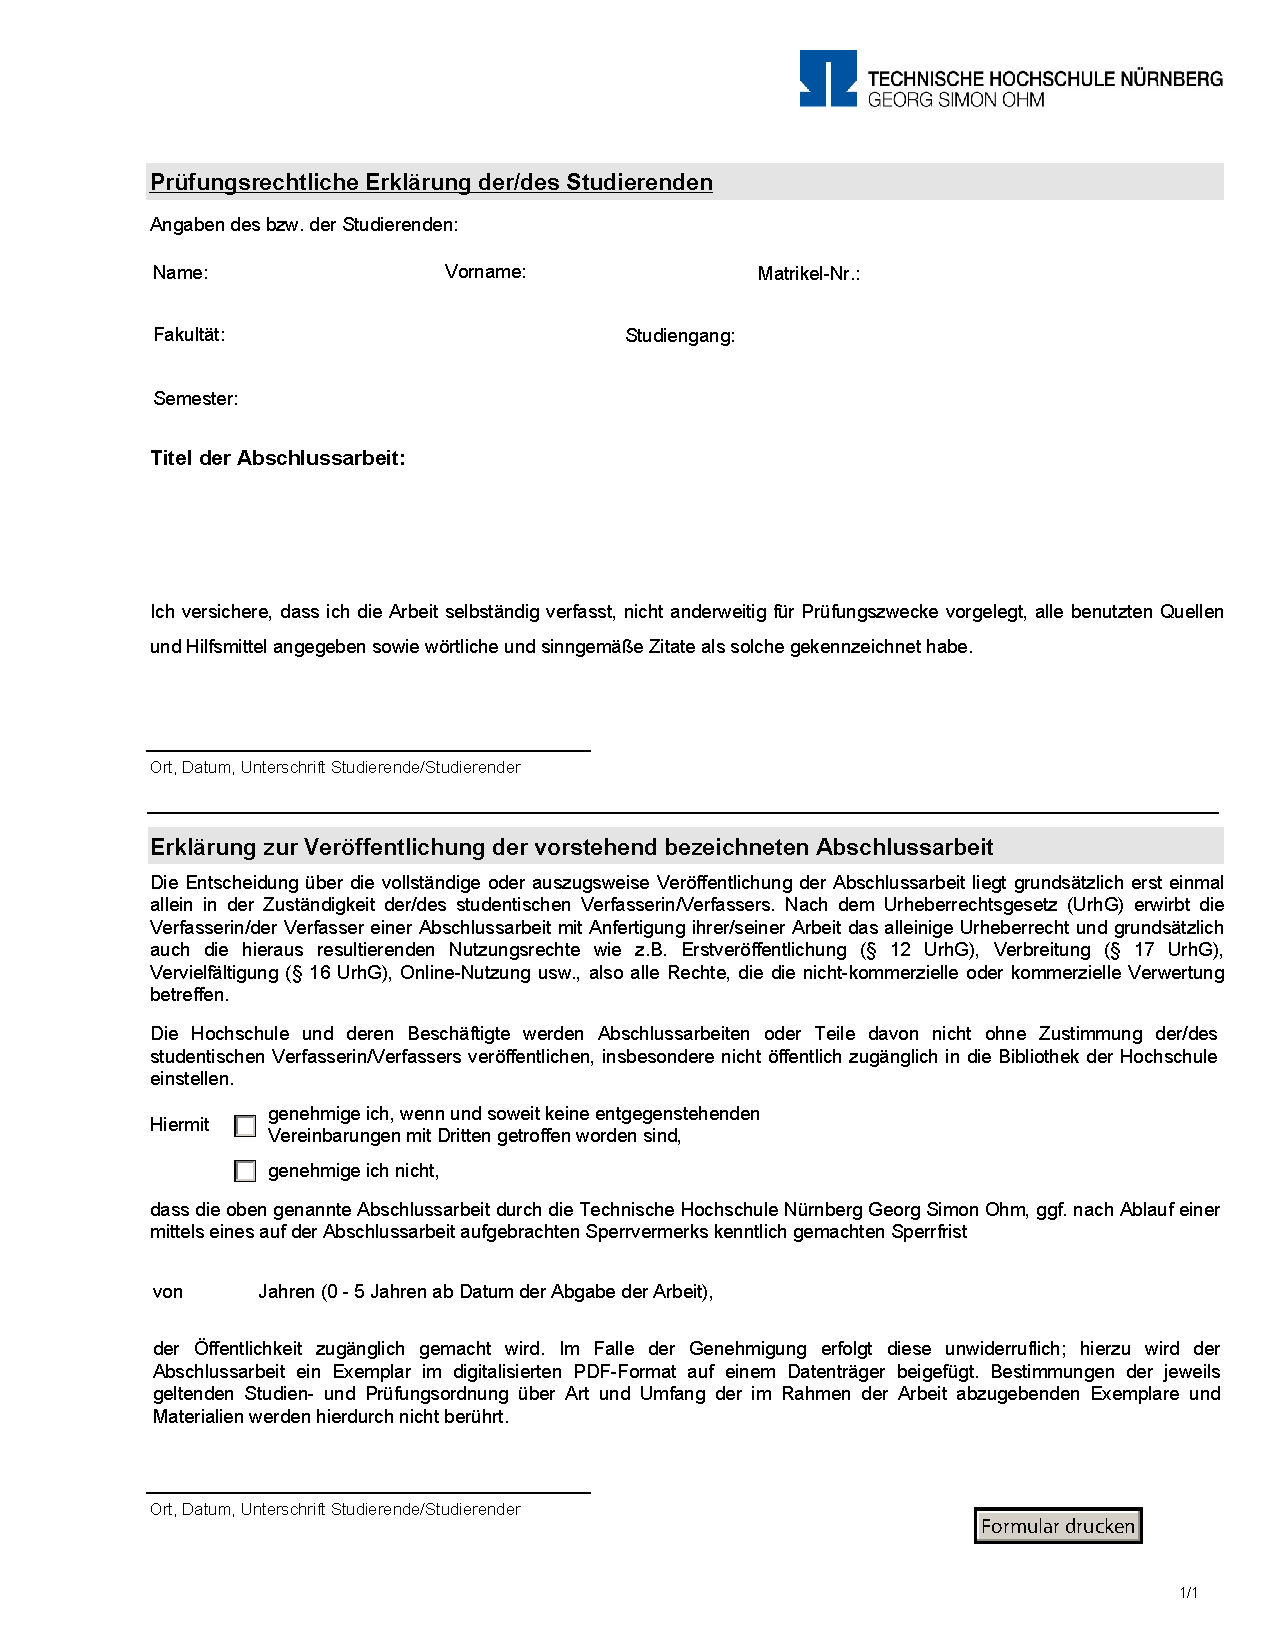
\includepdf{SB_0050_FO_Pruefungsrechtliche_Erklaerung_und_Erklaerung_zur_Veroeffentlichung_der_Abschlussarbeit_public.pdf}\cleardoublepage

\thispagestyle{empty}
\section*{Kurzdarstellung}
\label{sec:kurzdarstellung}
%Kurze Zusammenfassung der Arbeit, höchstens halbe Seite.
Open-Source-Projekte entwickeln Software, bei der der Quellcode frei verfügbar ist. Diese Communitys lassen automatisierte Tests gegen jede Code-Änderung laufen, um die bester Software-Qualität zu garantieren. 
Diese Tests sollen auf unterschiedlichen Architekturen laufen können. Es ist schwierig, Software für grundlegende Hardware ohne Zugriff darauf zu testen. Deshalb muss die in IBM Z verwendete s390x-Architektur für ausgewählte Open-Source-Projekte emuliert (nachgeahmt) und in die entsprechende CI/CD-Pipeline eingefügt werden. 
Das sollte mit schnellen Deployment-Methoden im Emulator QEMU durchgeführt werden. 
Kubernetes wird als containerisiertes Beispiel-Projekt als Grundlage für dafür eingeführte Anwendungen verwendet. Ein weiteres Open-Source-Projekt, Apache Cassandra, wird verwendet um Tests auf der Anwendungsschicht im Kubernetes-Stack zu repräsentieren. \\
Zusätzlich müssen die minimalen Systemanforderungen für die Einrichtung innerhalb der CI/CD-Infrastruktur beider Projekte wegen der Minimierung an Festplattenplatz, Memory und CPU-Verbrauch analysiert werden. \\
Zum Abschluss wird die automatische Emulation beider Projekte in die Test-Infrastruktur integriert, so dass diese Projekte für die s390x-Architektur von IBM Z Mainframes aktiviert sind. Allgemein soll diese Methode für weitere Open-Source-Projekte in der Zukunft wiederverwendet werden können.



\section*{Abstract}
\label{sec:abstract}

Open-source projects are developing software with freely available source code. These communities are running automated tests against every code change in order to guarantee the best software quality. 
These tests should be able to run on different architectures. It is difficult to test software for essential hardware without access. Therefore, the \gls{s390x} architecture used in IBM Z has to be emulated on x86 for chosen open-source projects and included in their \gls{CI/CD} pipeline. 
That should be executed with fast deployment methods in the \gls{emulator} QEMU. 
Kubernetes is used as a \gls{containerized} example project as the foundation for instituting applications. Another open-source project, Apache Cassandra, is applied to represent tests on the \gls{application layer} in the Kubernetes stack. \\
Additionally, minimal system requirements have to be analyzed for the setup inside of the CI/CD infrastructure of both projects concerning the minimization of disk space, memory and CPU usage for deployments. \\
Finally, the automated emulation of both projects will be integrated into the test infrastructure, so that these projects are enabled for the s390x architecture of \gls{IBM Z systems}. Overall, this method should be reusable for further open-source projects in the future.




\tableofcontents

\mainmatter
\chapter{Introduction}\label{ch:intro}


\blindtext

\section{Container Orchestration}

\blindtext

\subsection{Kubernetes}

Kubernetes\footnote{\url{https://kubernetes.io/}} is an open-source project for container orchestration. That is well known as K8s, too. This project was started by Google. A Kubernetes cluster has at least one Master node and one Worker node for high availability. This container platform portable for private und public clouds. Kubernetes is available as a managed platform by different cloud providers as same as different Kubernetes distributions exist to download or installations from scratch are possible. It is configurable with different container runtimes, as Docker\footnote{\url{https://www.docker.com/}}, Podman\footnote{\url{https://podman.io/}} or CRI-O\footnote{\url{https://cri-o.io/}} as examples. The Container Runtime Interface (CRI) is necessary for managing container images, the life cycle of container pods, networking and help functions\cite[~p.16]{Scholl2019}. 
\blindtext

\section{Mainframe Computers}

Mainframe computers are large computers. Some of them are part of the Z series\footnote{\url{https://www.ibm.com/it-infrastructure/z/hardware/}} by IBM. They are not only used as internet servers or for banking systems. They can handle large numbers of transactions in one second for e-commerce\cite[~p.56]{Tanenbaum2014}. Such Z systems do not use the well known x86 architecture. They are built with s390x. This architecture has been developed by IBM. It has been introduced in late 2000 and supported by the Linux Kernel since late 1999\cite[~p.15]{Block2019}. The traditional operating system for mainframes has been z\/OS. Linux is used as a base operating system for this Bachelor Thesis.


\blindtext

\section{Hardware Emulation}

Not everybody has access to expensive hardware or hardware with  specific architecture. Software should be able to run on most important hardware architectures. The solution for Software Developers is hardware emulation. You can test based on hypervisors with the hardware emulation whether the software is running correctly.
\blindtext

\section{Open Source Projects}
\blindtext

\subsection{And an even more important subsection}
\blindtext


\chapter{Emulation}\label{ch:emulation}

\section{QEMU}

QEMU is an open-source emulator introduced by Fabrice Bellard in the year 2003 and available in most Linux distributions now. It is embedded in different virtualization tools as KVM and XEN, too. QEMU is well tested and contains all the necessary features for emulations. 
You can emulate other architectures on different hardware. QEMU is a generic emulator for different system architectures. It can also be used for emulation of obsolete hardware \cite[~p.24]{Opsahl2013}. 
It has been extended for various architectures as x86, ARM, PowerPC, Sparc32, Sparc64, MIPS and s390x.
That is a processor emulator using binary translation \cite{Butt2011} which is executing and translating emulated instructions based on blocks. Each block comprises one entry and one exit point \cite[~p.5]{Wang2010}. 
The binary translation will be executed with the "Tiny Code Generator" (TCG) inside of QEMU. 
That is a small compiler replacing GCC because of unlimited releases and code changes. The TCG is converting the blocks of target instructions into a default intermediate form. 
Subsequently, it has to be compiled for the host or target architecture. 
If a binary for a new target architecture is necessary, the frontend of TCG will be converted while QEMU is ported to a new architecture. 
The TCG integrates new code for the new host architecture in the background then. It is also dedicated to improve performance with avoiding repeated translations by buffering already translated code \cite{Cota2017}. 
The TCG takes care of the emulation of the guest processor running as a thread launched by QEMU. The memory of a quest is allocated during launch and is mapped into the address space of the QEMU process \cite[~p.29]{Opsahl2013}.\\
It is possible to run unmodified guest operating systems. The open-source projects can use any Linux distribution as their base operating system then because QEMU is integrated as a default package. 
QEMU does not emulate the whole hardware. That is only possible for the CPU. QEMU is used for emulations in this Bachelor Thesis.

\section{Full System Emulation}

The Full System Emulation emulates a whole system with hardware, the operating system (with the kernel) and the userspace (with application processes). 
The system (hardware and operating system) will be translated unmodified. The benefit of system emulation (compared to user mode emulation) is that you can run privileged instructions \cite[~p.2]{Butt2011}. This feature enables the translation of unmodified  target code on the operating system.
Additionally, this emulation can be used as an application development platform where specific hardware is not available. 
System emulation with emulated hardware is slower than a real machine because instructions should be executed directly in the guest hardware.  But that has to be emulated in software. 
That implies multiple host instructions because of the translation for a single guest instruction as a result \cite[~p.1]{Tong2014}.
It is possible to reduce the supported and attached additional devices with special options. The deactivation of a graphic card can be specified with \textbf{-nographic} as an example. Afterwards, less hardware has to be emulated, which has given a better performance.  \\
System emulation benefits from the virtualization support as KVM. So most CPU operations are not required to emulate.

\section{User Mode Emulation}

The User Mode Emulation does not emulate the whole system. It is faster than the Full System Emulation because it does not engage so much hardware ressources. Application processes can be reproduced in QEMU with a minimal system for a specific application. 
This emulation type is working on a system call level. Therefore, the application has to be runnable as a process executable itself. The emulator is using the Linux kernel to emulate system signal calls then. That can be managed by mapping system calls of the target system to an equivalent system call on the host with threading (with a separate virtual CPU) \cite{QEMU}. This process does not require the emulation of the full  memory  management  unit \cite[~p.2]{Butt2011}.
The user-mode emulation can run directly non-privileged instructions or is using system calls to ask for a selected service from the operating system \cite[~p.2]{Butt2011}.


\section{Emulation of Alternative Architectures}

It is achievable to emulate alternative architectures on another hardware architecture. The package qemu-user-static has to be installed then, and the preferred architecture has to be registered in binfmt\_misc. binfmt\_misc is a kernel module. 
You can register other architectures within that, so multiple other architectures can be run on one host. 
Not only QEMU can be used for system emulation. Container technologies as Docker include an integrated QEMU compatibility as an additional emulation feature for building images for other architectures. 
This technology has got the name BuildX. Accordingly, a hybrid virtualization approach is practicable with different virtualization and emulation technologies as with QEMU and Docker together. In this case, an external Linux kernel will be integrated into QEMU, and the application can be mounted via a loaded Docker image in a hard disk image. \\
The initrd should match the Linux kernel and is optional. It is used to start an init process togeher with required test scripts.

\begin{figure}[H]
\centering
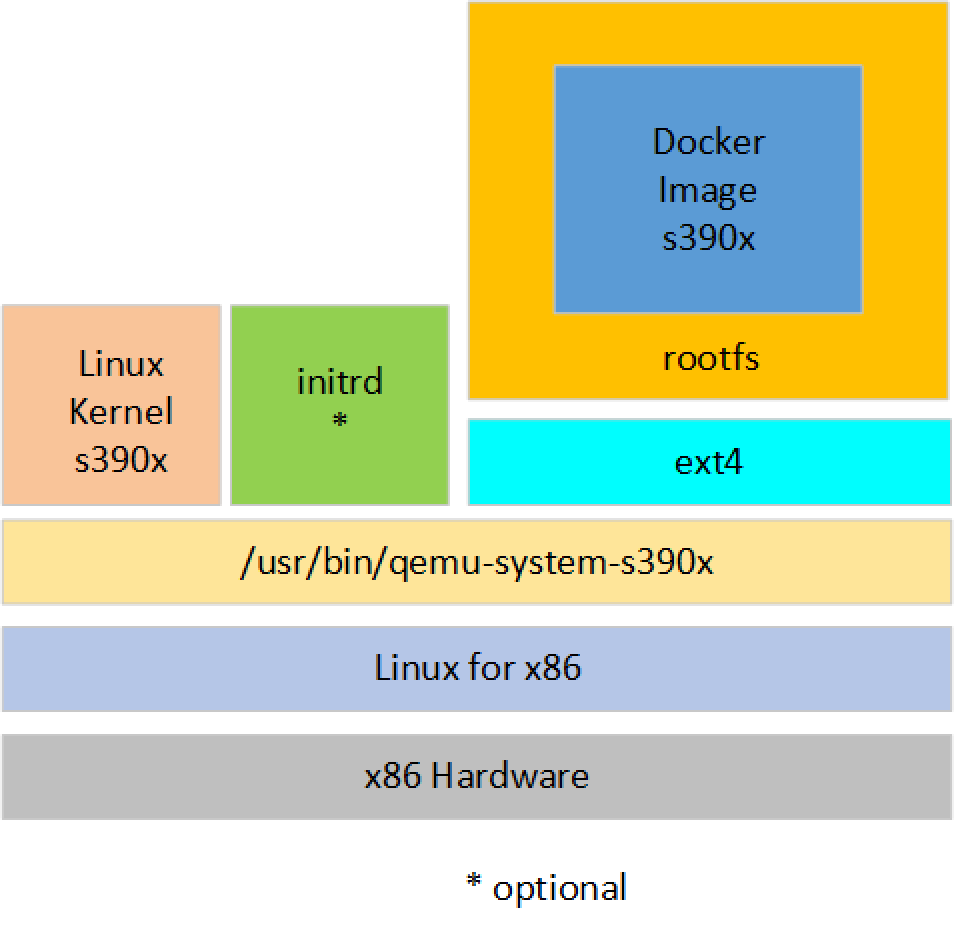
\includegraphics[height=9cm, width=9cm]{Qemu_setup}
 \caption{Emulation with QEMU}
    \label{QEMU_Emulation}
\end{figure}


\subsection{Binfmt\_misc}

Binfmt\_misc is a feature in the kernel which allows invoking almost every program by simply typing its name in the shell. That permits to execute user space applications such as emulators and virtual machines for other harware architectures. It recognises the binary-type by matching some bytes at the beginning of the file with a magic byte sequence. These executable formats have to be registered in the file \path{/proc/sys/fs/binfmt_misc/register}.\\
The structure of the configuration for the registration is the following: \\ \textbf{:name:type:offset:magic:mask:interpreter:flags} 

The \textbf{name} is the name of the architecture for the binary format. The \textbf{type} can be \textbf{E} or \textbf{M}. E is for executable file formats as .exe for example. M is used for a format identified by a \textbf{magic} number at an absolute \textbf{offset} in the file and the \textbf{mask} is a bitmask indicating which bits in the number are significant\cite{Slackware2020} (which is used in our case). 
The offset can be kept empty. The magic is a byte sequence of hexadecimal numbers. The \textbf{interpreter} is the program that should be invoked with the binary\cite{Guenther2020}. 
The path has to be specified for it. The field \textbf{flags} is optional. It checks different aspects of the invocation of the interpreter. The \textbf{F} flag is necessary in our case for "fix binary". 
That supposes that a new binary has to be spawned if the misc file format has been invoked.\\
In this way, it is possible to register another system architecture (s390x on x86) on the host system and it is realizable to emulate the other architecture afterwards. \\
The necessary command for s390x registration can be found under \ref{Qemu-S390-Registration}.
The package \textbf{binfmt-support} has to be installed first for using this kernel feature. 

\subsection{Qemu-user-static}

The package \textbf{qemu-user-static}\footnote{\url{https://github.com/multiarch/qemu-user-static}} enables the execution of multi-architecture container emulation based on \textbf{binfmt\_misc} with \textbf{QEMU}. This package provided by various Linux distributions includes a set of binfmt configurations for various architectures together with an amount of statically compiled QEMU emulators that alternative architectures can run on another architecture \cite{Yang2019}. When building for one new architecture, static binaries are important because of the possibility of an "exec init error" without them. \\
The installation contains emulators for all available architectures supported by the QEMU project incl. s390x aligned with the specific host architecture. In this manner, you can build and run a binary for different architectures on the same host (see \ref{Optimized-Qemu-Command} Optimized Qemu Command). That is the base for BuildX by Docker, too.

\subsection{BuildX}

As mentioned above, Docker is using QEMU for emulations with BuildX\footnote{\url{https://github.com/docker/buildx}}. That is an integrated "experimental Feature" since version Docker 19.03. That implies that it is not enabled as default because it is very new and for experiments. It has to be activated with \lstinline!DOCKER_CLI_EXPERIMENTAL=enabled! (see \ref{Qemu-S390-Registration} Registration of Qemu-S390x). The disadvantage of the provided BuildX inside of Docker is that you do not receive the up-to-date version of BuildX. There is a version with a more detailed output and better working with an additional \textbf{buildx} behind \textbf{docker build}. This version can be cloned from \url{https://github.com/docker/buildx} and installed with \textbf{make install}. \\
In general, BuildX is a Docker CLI plugin for expanding the "docker build" command. That includes the possibility of multi-architecture builds and exceptional output configuration. That involves not only the upload possibility to your local docker registry (see the output of \textbf{docker images}). That includes the output of "docker build" (which creates a docker image based on the requirements and installations in the used Dockerfile) into a local directory, a tar archive or a public registry on Docker Hub. Docker Hub is the most used and maintained registry for Docker images. \\
The \textbf{Dockerfile} is using the requirements by the base docker image in the FROM command on top of the Dockerfile together with installations and configurations executed by all RUN commands or attached scripts with the command ADD. The \textbf{-t} flag is adding a special name as a tag under \textbf{docker images}.
The special architecture for multi-architecture\ref{MultiArchitectureImages} builds can be specified with the additional option \textbf{--platform}.
The option \textbf{build create} provides the option to create different build instances for multiple build combinations of architectures.

\subsection{Multi-Architecture Images}\label{MultiArchitectureImages}

Default Linux distribution providers have to package their software for different system architectures because of different required drivers included in the Linux kernel and dependecies to these.
That is the reason that Docker images have to be built equally for different architectures. That can be performed with different base images for the respective architectures or with multi-arch images. 
It is possible to use one Dockerfile for different architectures then. One example for such a multi-arch Docker image is adoptopenjdk/adoptopenjdk8 based on Ubuntu\footnote{\url{https://github.com/AdoptOpenJDK/openjdk-docker/blob/master/8/jdk/ubuntu/Dockerfile.hotspot.nightly.full}}. In this case hardware dependencies are selected with \lstinline!dpkg --print-architecture! and included as ARCH into the different cases for downloading the relevant tar archive of OpenJDK:
\begin{figure}[H]
\centering
\begin{boxedverbatim}
RUN set -eux; \
    ARCH="$(dpkg --print-architecture)"; \
    case "${ARCH}" in \
       aarch64|arm64) \
         ESUM='2c6540ff8ea3d89362fd02143b24303e2359be249a6be6cb7e6580472686d863'; \
         BINARY_URL='https://github.com/AdoptOpenJDK/openjdk8-binaries/releases/
         download/jdk8u-2020-08-05-08-20/OpenJDK8U-jdk_aarch64_linux_hotspot_2020-
         08-05-08-20.tar.gz'; \
         ;; \
       armhf|armv7l) \
         ESUM='3c57c121415ef721ba9c73dfa809cd2f689d7369ef3d92d055f7c7c81ed2d697'; \
         BINARY_URL='https://github.com/AdoptOpenJDK/openjdk8-binaries/releases/
         download/jdk8u-2020-07-31-04-43/OpenJDK8U-jdk_arm_linux_hotspot_2020-07-
         31-04-43.tar.gz'; \
         ;; \
       ppc64el|ppc64le) \
         ESUM='668972e8d6d0815c03b32dac3f5c663453b4b0842938d13cfb0c1232a26a8087'; \
         BINARY_URL='https://github.com/AdoptOpenJDK/openjdk8-binaries/releases/
         download/jdk8u-2020-08-05-08-20/OpenJDK8U-jdk_ppc64le_linux_hotspot_2020-
         08-05-08-20.tar.gz'; \
         ;; \
       s390x) \
         ESUM='045aa287c48fd84eef19f2828ed1d15d27059a9328f5ca2cc91f6d42489af956'; \
         BINARY_URL='https://github.com/AdoptOpenJDK/openjdk8-binaries/releases/
         download/jdk8u-2020-08-05-08-20/OpenJDK8U-jdk_s390x_linux_hotspot_2020-
         08-05-08-20.tar.gz'; \
         ;; \
       amd64|x86_64) \
         ESUM='c26124b14c6a42d89278d3ce108b43c1210a317aba0163d985c06a79a695a174'; \
         BINARY_URL='https://github.com/AdoptOpenJDK/openjdk8-binaries/releases/
         download/jdk8u-2020-08-05-08-20/OpenJDK8U-jdk_x64_linux_hotspot_2020-08-
         05-08-20.tar.gz'; \
         ;; \
       *) \
         echo "Unsupported arch: ${ARCH}"; \
         exit 1; \
         ;; \
    esac; 
\end{boxedverbatim}
 \caption{Multi-Arch Image AdoptOpenJDK 8}
    \label{AdoptOpenJDK-Multi-Arch}
\end{figure}

You can see all URLs for arm64, armv7l, ppc64le, s390x and x86 in this case. This RUN command in the Dockerfile is using the architecture given by the option \\
\lstinline!--build-arg ARCH=s390x! \\
as an example in the \lstinline!docker build! command or the \lstinline!--platform! option will be used with BuildX.
\lstinline!Docker build! is stacked against BuildX, because only one image can be built with one command.
Buildx provides the possibility to consign different architectures (comma separated) to the platform option. Thereby, one command can build multiple images for different architectures.

\section{File Systems}\label{FileSystems}

Docker is using the Union File System which is not compatible with QEMU. \\
QEMU can integrate only hard disk formats for default Linux file systems as ext2, ext3, ext4, XFS and Btrfs. 
The driver virtio\_blk is used to mount external file systems and emulates read/write in the physical block device\cite{Barboza2018}. Following it, is possible to integrate and start nonnative systems in QEMU. 
Docker is advantageous to setup and start systems fast. 
It would be nice to integrate the docker file system into QEMU. After building a docker image, it is realizable to export the file system into a directory with the name \textbf{rootfs} with the command \\ 
\lstinline!docker export $(docker create initrd-s390x) | tar -C "rootfs" -xvf -!. \\

Linux has got the feature that it is adventitious to reformat directories for file systems and to copy/ mount content into this one. Reformatting the default docker file system UnionFS to another one as ext4 for example can be done then. \\
QEMU is accepting the new file system as a block device for the guest system then. The default path to the mounted file system as a hard disk is \path{/dev/vda} as the first partition \cite[~p.22]{White2020}.

\subsection{UnionFS}\label{UnionFS}

Docker does not use any default Linux file system. 
Docker images are based on the Union File System (UnionFS) \cite[~p.21]{Ashraf2015}. 
This file system is using different file system layers with grouping directories and files in branches. 
The first layer is the typical Linux boot file system with the name bootfs. 
That performs the same as in a Linux virtualization stack with using memory at first and unmounting to receiving RAM free by the initrd disk image. 
So the bootfs can be used inside of another Linux file system to mount in an virtualization stack for a successful boot process with QEMU.
The next layer contains the base image with the operating system given by the "FROM" command.
Then every docker command inside of the Dockerfile is adding an additional layer with the installation of applications or building binary files.
That is the reason that every executed docker command is receiving an own id in the disk memory during the build process.
Every separate docker command is using his own disk space. So a docker image can grow really fast.
It is reasonable to compress so much as possible of different routines into one docker command. 
All sizes of different docker layers will exist continuously inside of the new file system.

\begin{figure}[H]
\centering
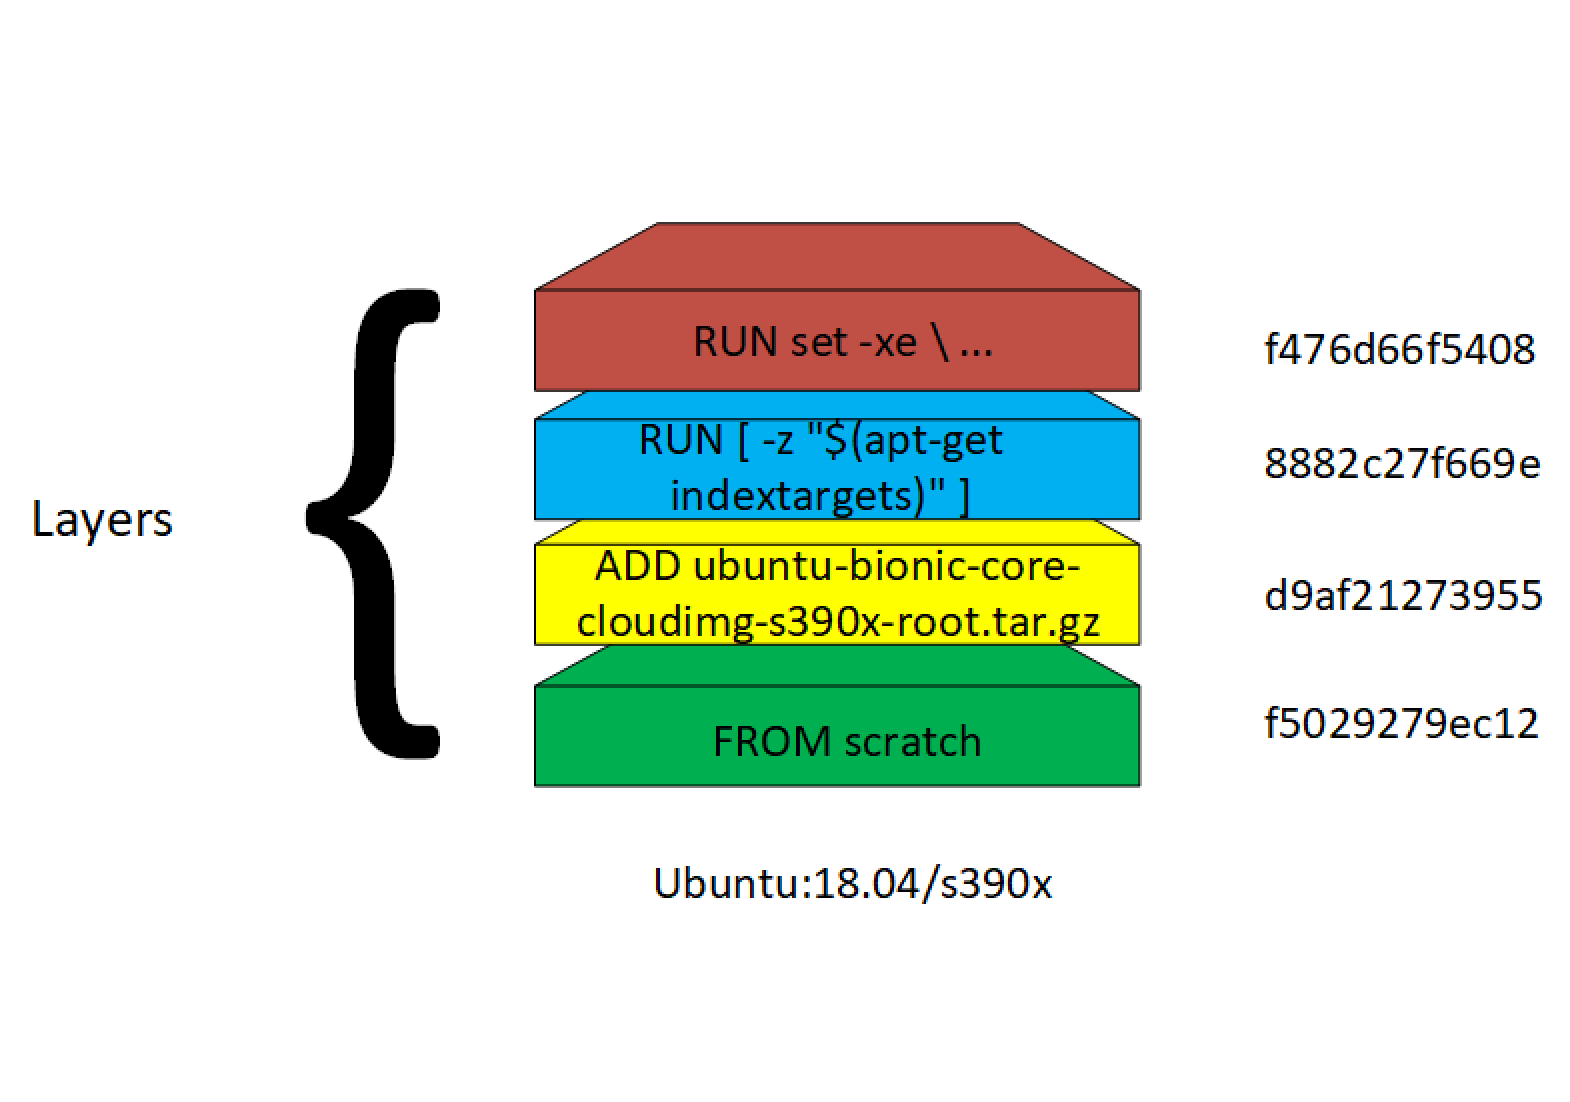
\includegraphics[width=\textwidth]{UnionFS}
 \caption{Union File System}
    \label{UnionFS}
\end{figure}

\subsection{Ext4}

Ext4 is a journaling file system (the same as ext3). The journal is registering transactional all changes on the operating system with meta data.
So no data  are lost after a system failure. They can be restored based on the journal without a save procedure by the user.
Such journal file systems in the ext file system family are working with blocks \cite[~p.20]{Seufert2015}.
The journal is splitted into the journal super block, descriptor blocks, commit blocks and revoke blocks.
The super block contains all meta data of the journal. Descriptor blocks include the special destination adress and a sequence number. 
Flex groups can combine multiple group blocks - inode bitmaps, inode tables and data blocks - to one logic block group. All data from inodes are only saved in the first flex group then. 
So the search for files is more powerful because meta data are allocated at one place.\\
All meta data from the journal can be relocated in inodes because changes of file system meta data are registered, too. \\
The difference to the journal in ext3 are the option writing asynchronous commit blocks and additional check sums for journal transactions \cite[~p.28]{Seufert2015}.

Ext4 provides a better performance than ext3. 
This file system can be formated with mkfs.ext4 which is available in every Linux distribution.
This tool is creating a group despriptor table for further group descriptors what allows an expanding of the file system. The file system can grow a maximum of the multiple 1024 of his existing size because of the saved space \cite[~p.21]{Seufert2015}. \\

Another feature of ext4 is the possibility of inline files and inline directories. So small files and directories can be saved directly in inodes instead of data blocks. From this follows less disk space consumption \cite[p.24]{Seufert2015}.

\begin{figure}[H]
\centering
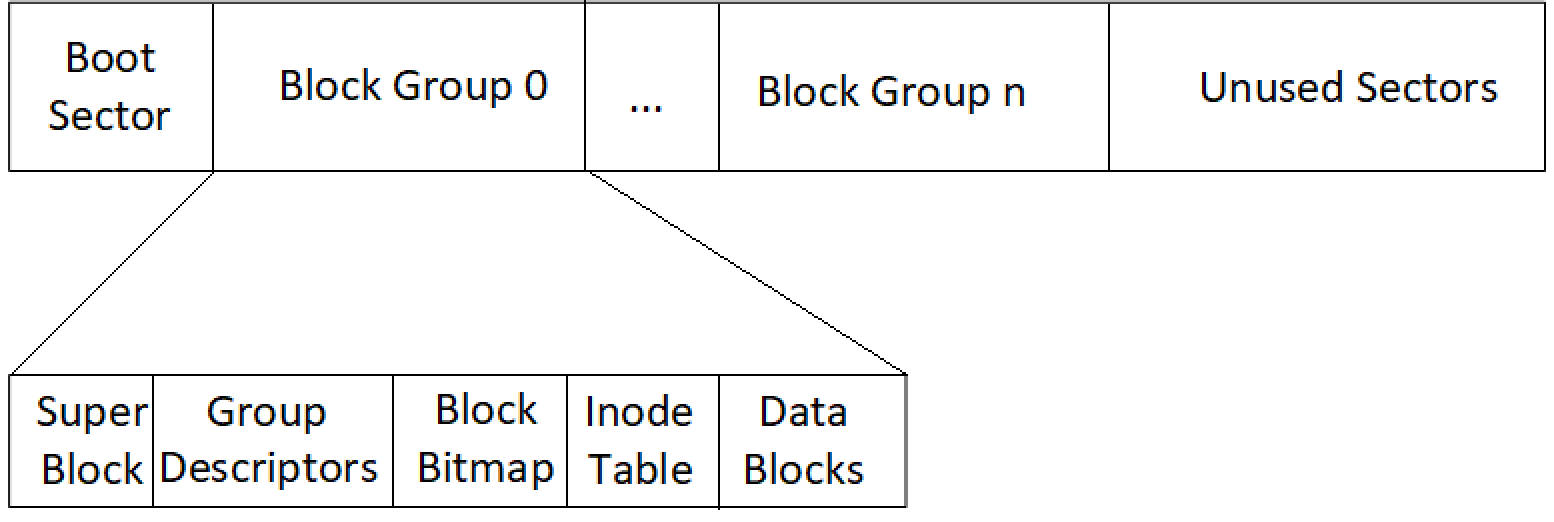
\includegraphics[width=\textwidth]{Ext4}
 \caption{Ext4}
    \label{Ext4}
\end{figure}

\subsection{Mounting an External File System}

In \ref{FileSystems}"File Systems" is described how to export a Docker file system into a directory. That has got the format of the \ref{UnionFS}UnionFS at this moment. QEMU contains the beneficial tool \textbf{qemu-img} for creating loadable images of file systems. These require the minimal size of the docker image. The output of the size is given by \lstinline!docker images | grep ${id}!. QEMU understands only rounded numbers. Therefore, that has to be rounded up to a full number. Cassandra is using the command \\
\lstinline!qemu-img create -f raw cassandra.img 2G! (see \ref{RunningDockerImage}"Running the Docker Image") \\
for a Docker image size about 1.2G then. Firstly, cassandra.img is empty. The content of \textbf{rootfs} has to be transferred into this image file. But QEMU does not know UnionFS as a file system. That is the reason for formatting cassandra.img with \lstinline!mkfs.ext4 -F cassandra.img! to ext4. Writing into cassandra.img is only executible if the image is mounted into a directory under \path{/mnt/} with \\
\lstinline!mount -o loop cassandra.img /mnt/rootfs!. \\ 
In the next step the content of the file system directory can be copied into \path{/mnt/rootfs/} with \\ 
\lstinline!cp -r rootfs/* /mnt/rootfs/.!. \\ 
Then all data of the Docker image are saved into cassandra.img because it is mounted into \path{/mnt/rootfs/}. The image cassandra.img is usable for deployments with \textbf{qemu-system-s390x} (see \ref{RunCassandra} Run Cassandra) at the end. 
\chapter{Continuous Integration}\label{ch:ci_cd}

\Blindtext

\chapter{Cassandra}\label{ch:cassandra}

\Blindtext

\usepackage{verbatim}

\chapter{Kubernetes}\label{ch:kubernetes}

\section{Overview}

Kubernetes is a container platform for high availability clusters.
There exist plugins for integration tests for Kubernetes with the name kubetest\footnote{\url{https://kubetest.readthedocs.io/en/latest/}}. They contain conformance tests, as e2e tests (end-to-end), too.
That can be all built and executed on the system. Therefore, a Dockerfile for setting up Kubernetes and building tests with go is necessary. The problem is, that 2 big Github repositories have to be cloned and integrated into the docker image. That is using a lot of space. The solution is using a multi staging Dockerfile. 
So 2 different Dockerfiles are used in one Dockerfile and one is used for building. The other one is used for the installation and testing with built tests. At the end the size of the docker image has got only the size of the test image unimportant of the repository size in the mother Dockerfile.

\section{Multi Staging}

A multi-staging Dockerfile is using different systems in one Dockerfile for different stages. These systems are receiving special names as indicators with \ldq AS \rdq behind the \ldq FROM \rdq with the base image name. 
Default this feature is used for building applications in one stage and executing the copied application in another stage. The same counts for clonining Github repositories and building binary files based on it. On this way a lot of space is saved.
At the end the docker image has got only the size of the executing system with the application file (without all the code). 
That is an \rdq experimental feature \rdq at the moment. Therefore the \textbf{experimental flag} is necessary to export or set before using it. 

\section{Installation}

Kubernetes needs a lot of packages for running and for tests. That will be all installed with the RUN command.
\url{apt.kubernetes.io} has got later packages as the Ubuntu repository. Therefore this repository has to be added to Ubuntu. kub-build is the name of the mother Dockerfile to be able to copy needed files and directories from there.

\begin{verbatim}[frame=single]
FROM s390x/ubuntu:18.04 AS kub-build
 
# The author
MAINTAINER Sarah Julia Kriesch <sarah.kriesch@ibm.com>

#Installation
RUN echo "Installing necessary packages" && \
apt-get update && apt-get install -y \
apt-transport-https \
apt-utils \
systemd \
curl \
git \
ca-certificates \
gnupg-agent \
software-properties-common \
&& curl -s https://packages.cloud.google.com/apt/doc/apt-key.gpg | apt-key add - \
&& echo "deb https://apt.kubernetes.io/ kubernetes-xenial main" 
> /etc/apt/sources.list.d/kubernetes.list \
&& apt-get update && apt-get install -y \
docker.io \
kubelet \
kubeadm \
&& apt-mark hold kubelet kubeadm kubectl \
&& apt-get clean \
&& rm -rf /var/lib/apt/lists/* /tmp/* /var/tmp/* \
&& systemctl enable docker 
\end{verbatim}

\section{Building latest Go}

There were some issues with older Go versions as 1.10 during building tests for Kubernetes. Therefore a higher version (min. 1.13) should be used. It is recommended to use the latest go version for latest Kubernetes tests. It is possible to receive the version number of the latest go release with the command \shellcmd{curl \url{https://golang.org/VERSION?m=text}}. This version number has to be included before linux-s390x.tar.gz for downloading the special s390x archive from the go directory by \url{dl.google.com}. Directories for bin, pkg and src have to be created after extracting this tar archive in the \path{/root/} directory. \\

The environment variables for GOROOT, GOPATH and PATH have to be set with ENV on the top of the Dockerfile for successful builds later. PWD is added because Github repositories have to be cloned to this directory.

\begin{verbatim}[frame=single]
ENV GOROOT=/root/go
ENV GOPATH=/root/go
ENV PATH=$GOPATH/bin:$PATH
ENV PATH=$PATH:$GOROOT/bin
ENV PWD=/root/go/src/

#Installation of latest GO
&& echo "Installation of latest GO" && \
curl "https://dl.google.com/go/$(curl https://golang.org/VERSION?m=text).linux-s390x.tar.gz" \
| tar -C /root/ -xz \
&& mkdir -p /root/go/{bin,pkg,src} \
\end{verbatim}

\section{Building tests}
After a successful installation of go, it is possible to build and install the Kubernetes test environment.
At first the directory k8s.io has to be created because kubernetes-tests are looking for this directory as a mother directory. The repository test-infra by the Kubernetes project has to be cloned to there. Inside of this test-infra directory kubetest can be installed with \textbf{go install}. That is downloading all available Kubernetes-Tests. So you can use them to test the own Kubernetes cluster and the used software. \\

The most important tests for the Kubernetes community have got the name conformance tests. These tests certifies the software to comply regular standards. Only with complying these standards, Kubernetes software is allowed to become Kubernetes certified\footnote{https://github.com/cncf/k8s-conformance}. 
These conformance tests are executed with e2e.test. This test file can be built with make inside of the kubernetes repository. Therefore this repository has to be cloned to k8s.io, too.


\begin{verbatim}[frame=single]
&& cd $PWD \
#Clone test-infra
&& mkdir -p $GOPATH/src/k8s.io \
&& cd $GOPATH/src/k8s.io \
&& git clone https://github.com/kubernetes/test-infra.git 
/root/go/src/k8s.io/test-infra \
&& cd /root/go/src/k8s.io/test-infra/ \
#Install kubetest
&& GO111MODULE=on go install ./kubetest \
#Build test binary
&& git clone https://github.com/kubernetes/kubernetes.git 
/root/go/src/k8s.io/kubernetes \
&& cd /root/go/src/k8s.io/kubernetes/
 
CMD make WHAT="test/e2e/e2e.test vendor/github.com/onsi/ginkgo/ginkgo cmd/kubectl"
\end{verbatim}

\Blindtext

\chapter{Outlook}\label{ch:outlook}

\Blindtext

\chapter{Summary}\label{ch:summary}

\Blindtext

\makeglossaries
\printglossary[style=altlist, title=Glossary, nonumberlist]
\newglossaryentry{glos:ML}{name=Maschinelles lernen, description={Maschinelles Lernen beschreibt Algorithmen, welche ...}}

\deftranslation[to=English]{Acronyms}{dds}
\printglossary[type=\acronymtype,style=long,title=Shortwords]

% remove if not needed
\appendix
\chapter{Supplemental Information}\label{app:supplemental-information}

\section{Circle CI configuration for Apache Cassandra}\label{CircleCI}
\begin{boxedverbatim}
jobs:
  build-docker-image:
    working_directory: ~/s390x
    docker:
      - image: Dockerfile
    steps:
      - attach_workspace:
          at: .
      
      - run: 
            name: Build for s390x
            command: docker build buildx --platform=linux/s390x --squash \
                    -t cassandra:s390x .
      - docker/check:
         registry: $DOCKER_REGISTRY 
  prepare-kernel:
    steps:
        - run:
              name: Fetching the Linux kernel
              command: |
                      mkdir ~/s390x/kernel-bionic; debootstrap --include=linux-generic \
                      --arch=s390x --variant=minbase bionic kernel-bionic \
                      http://ports.ubuntu.com
        - store_artifacts:
              path: ~/s390x/kernel-bionic/boot/vmlinuz-4.15.0-20-generic
        - persist_to_workspace:
                  root: .
                  paths:
                      - .
        
\end{boxedverbatim}

\begin{boxedverbatim}
  prepare-filesystem:
    working_directory: ~/s390x
      steps:
        - attach_workspace:
                  at: .
        - run:
              name: Creating a ext4 filesystem with integration of the Cassandra image
              command: |
                      mkdir rootfs; qemu-img create -f raw cassandra-s390x.img \
                      $(docker images | grep 'cassandra:s390x' | \
                      awk '{print int($7+0.5)"G"}'); \
                      docker export $(docker create cassandra:s390x)| \
                      tar -C "rootfs"-xvf -;  mkfs.ext4 -F cassandra-s390x.img;\
                       mount -o loop cassandra-s390x.img /mnt/rootfs; \
                      cp -r rootfs/* /mnt/rootfs/.
        - store_artifacts:
              path: ~/s390x/cassandra-s390x.img
  test:
  working_directory: ~/s390x
    steps:
      - attach_workspace:
                  at: .
      - run:
             name: Run test with QEMU
             command: |
                     /usr/bin/qemu-system-s390x -kernel vmlinuz-4.15.0-20-generic \
                     -m 4G -M s390-ccw-virtio -nodefaults -device sclpconsole,\
                     chardev=console -parallel none -net none -chardev stdio,\
                     id=console,signal=off,mux=on -mon chardev=console \
                     -nographic -smp 3 -hda cassandra-s390x.img \
                     --append ’root=/dev/vda rw console=ttyS0 rdinit=/bin/bash’  
workflows:
    version: 1
    build-test:
      jobs:
        - prepare-kernel
        - build-docker-image
              requires: 
                  - prepare-kernel
        - prepare-filesystem
              requires: 
                  - build-docker-image
        - test
             requires:
                 - prepare-kernel
                 - prepare-filesystem
\end{boxedverbatim}

\backmatter
\listoffigures
\cleardoublepage

\listoftables
\cleardoublepage

\renewcommand{\lstlistlistingname}{List of Listings}  % change for German thesis
\lstlistoflistings
\cleardoublepage

\bibliographystyle{wmaainf}
\bibliography{refs}

\end{document}
